\documentclass[11pt]{article}
\usepackage[margin=1in]{geometry}
\usepackage{amsmath,amssymb}
\usepackage{enumitem}
\usepackage{booktabs}
\usepackage{xcolor}
\usepackage{listings}
\usepackage{graphicx}
\setlength{\parindent}{0pt}
\setlength{\parskip}{4pt}
\setlist[enumerate]{label=(\alph*), leftmargin=*, itemsep=8pt}
\lstset{language=R,basicstyle=\ttfamily\small,keywordstyle=\color{blue!70!black},commentstyle=\color{gray},frame=single,rulecolor=\color{gray!60},backgroundcolor=\color{gray!6},xleftmargin=4pt,xrightmargin=4pt,aboveskip=6pt,belowskip=4pt,showstringspaces=false,columns=fullflexible,keepspaces=true}
\newcommand{\chk}[1]{{\color{red}#1}}% red = simulation value to confirm in R

\title{STT 465 -- Homework 2: Single-Parameter Bayesian Models}
\author{Mihir Patel}
\date{October 2026}
\begin{document}
\maketitle

%================================================================
\section*{Question 1: Bernoulli-Beta Posterior}
Let $s=\sum x_i = 18$, $n=25$, so $n-s=7$.
\begin{enumerate}
\item $L(\omega\mid x)=\prod_{i=1}^{25}\omega^{x_i}(1-\omega)^{1-x_i}\propto \omega^{18}(1-\omega)^{7}.$

\item The prior is $\pi(\omega)\propto\omega(1-\omega)$. By Bayes' theorem
\[
\pi(\omega\mid x)\propto L(\omega\mid x)\pi(\omega)\propto\omega^{18+1}(1-\omega)^{7+1}=\omega^{20-1}(1-\omega)^{9-1},
\]
the kernel of a Beta distribution, so $\omega\mid x\sim \mathrm{Beta}(20,9)$.

\item For $\mathrm{Beta}(\alpha,\beta)$, $E=\alpha/(\alpha+\beta)$. In general the posterior is $\mathrm{Beta}(a+s,\,b+n-s)$, so
\[
E[\omega\mid x]=\frac{a+s}{a+b+n}=\frac{2+18}{2+2+25}=\frac{20}{29}\approx 0.6897.
\]

\item Mode $=\dfrac{\alpha-1}{\alpha+\beta-2}=\dfrac{19}{27}\approx 0.7037$. Median: \texttt{qbeta(0.5, 20, 9)} $\approx 0.6941$.

\item \begin{lstlisting}
1 - pbeta(0.70, 20, 9)     # equivalently pbeta(0.70, 20, 9, lower.tail = FALSE)
\end{lstlisting}
$P(\omega>0.70\mid x)\approx 0.4725$.
\end{enumerate}

%================================================================
\section*{Question 2: Prior Sensitivity and Bayesian Updating}
Here $n=21$, $x=18$ (successes), $n-x=3$.
\begin{enumerate}
\item Posterior $\propto\omega^{18}(1-\omega)^{3}\cdot\omega^{0}(1-\omega)^0$, so $\omega\mid x\sim\mathrm{Beta}(1+18,\,1+3)=\mathrm{Beta}(19,4)$.
\item Posterior $\propto\omega^{18}(1-\omega)^{3}\cdot\omega^{3}(1-\omega)^{-0.1}$, so $\omega\mid x\sim\mathrm{Beta}(4+18,\,0.9+3)=\mathrm{Beta}(22,3.9)$.
\item The posterior is $\mathrm{Beta}(a+x,b+n-x)$, so
\[
E[\omega\mid x]=\frac{a+x}{a+b+n}=\frac{a+b}{a+b+n}\cdot\frac{a}{a+b}+\frac{n}{a+b+n}\cdot\frac{x}{n}.
\]
The first term is the prior mean $a/(a+b)$ weighted by $(a+b)/(a+b+n)$ (the prior ``sample size'' share); the second is the sample proportion $x/n$ weighted by $n/(a+b+n)$ (the data's share). The posterior mean is a weighted average of prior mean and MLE.
\item Prior A: $19/23\approx0.8261$. Prior B: $22/25.9\approx0.8494$. They differ because Prior B has prior mean $4/4.9\approx0.816$ and prior weight $a+b=4.9$ versus $2$ for Prior A (prior mean $0.5$). Both are pulled from the sample proportion $18/21\approx0.857$ toward their prior mean, but A is pulled more, since it has a lower prior mean and a less informative prior, while B sits closer to the data. With $n=21$ the data dominate, so the difference is small.
\item \begin{lstlisting}
w <- seq(0, 1, length.out = 1000)
plot(w, dbeta(w, 19, 4), type = "l", lwd = 2, col = "blue",
     xlab = expression(omega), ylab = "Posterior density")
lines(w, dbeta(w, 22, 3.9), lwd = 2, col = "red", lty = 2)
abline(v = 18/21, lty = 3)
legend("topleft", c("Prior A: Beta(19,4)", "Prior B: Beta(22,3.9)", "18/21"),
       col = c("blue","red","black"), lty = c(1,2,3), lwd = 2)
\end{lstlisting}
\begin{center}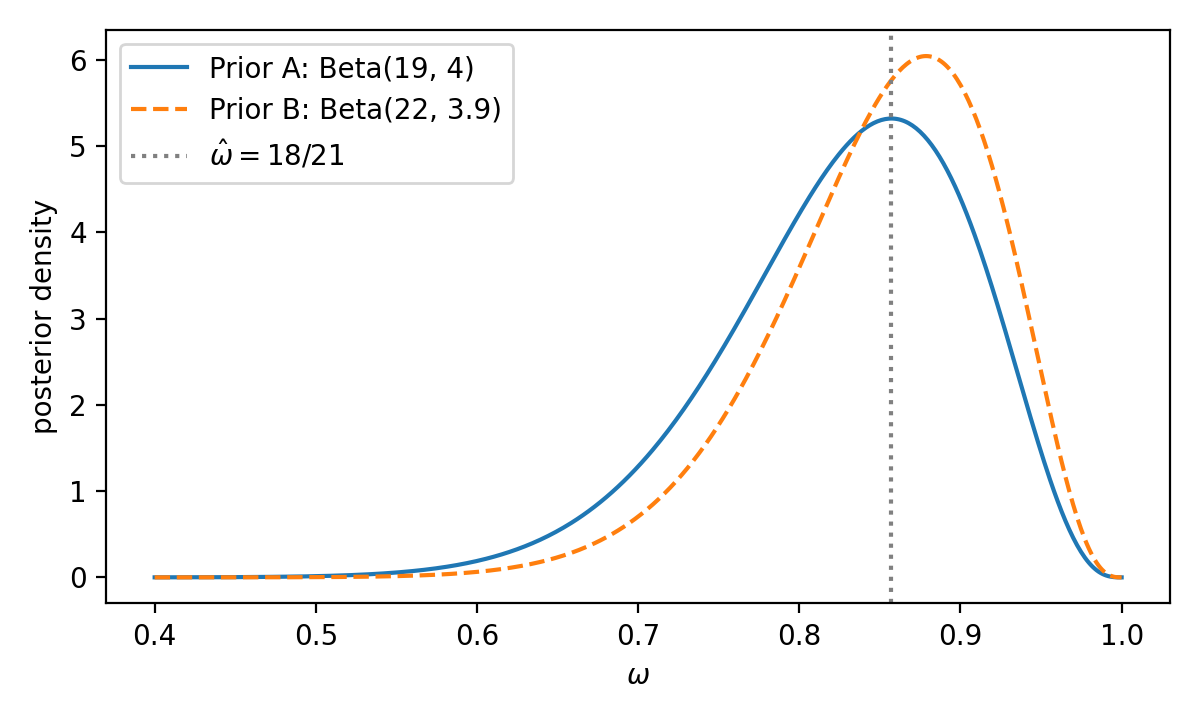
\includegraphics[width=0.6\linewidth]{q2e.png}\end{center}
Both posteriors are concentrated around 0.8--0.9 and overlap heavily. Posterior B is shifted slightly right (closer to $18/21$), while Prior A's posterior has slightly more mass at lower values and is slightly wider. With 21 observations the choice of prior matters little.
\end{enumerate}

%================================================================
\section*{Question 3: Credible Intervals and HPDI}
\begin{enumerate}
\item \begin{lstlisting}
qbeta(c(0.025, 0.975), shape1 = 22, shape2 = 4)
\end{lstlisting}
The 95\% equal-tailed interval is $[0.6878,\ 0.9546]$.
\item Given the model, prior and observed data, there is a 95\% posterior probability that $\omega$ lies in $[0.688,0.955]$. Unlike a frequentist confidence interval, $\omega$ is treated as random and the interval as fixed once the data are observed.
\item \begin{lstlisting}
library(HDInterval)
set.seed(1)
omega_post <- rbeta(10000, shape1 = 22, shape2 = 4)
hdi(omega_post, credMass = 0.95)
\end{lstlisting}
The 95\% HPDI is approximately $[\chk{0.705,\ 0.964}]$ (exact HPD from the density: $[0.709,\ 0.967]$).
\item The equal-tailed interval has length $0.2668$; the HPDI has length about $0.26$ (exact $0.2573$). The HPDI is shorter.
\item The equal-tailed interval leaves 2.5\% in each tail, while the HPDI is the shortest interval with 95\% mass, containing the highest-density points. For a symmetric unimodal posterior they coincide. $\mathrm{Beta}(22,4)$ is left-skewed, with a long lower tail and a steep upper end, so the HPDI shifts right and trims the low-density lower tail.
\end{enumerate}

%================================================================
\section*{Question 4: Comparing Two Population Proportions}
\begin{enumerate}
\item With uniform priors, $\omega_x\mid x\sim\mathrm{Beta}(1+437,\,1+543)=\mathrm{Beta}(438,544)$ and $\omega_y\mid y\sim\mathrm{Beta}(1+398,\,1+422)=\mathrm{Beta}(399,424)$, independently.
\item $E[\omega_x\mid x]=438/982\approx0.4460$; $E[\omega_y\mid y]=399/823\approx0.4848$.
\item \begin{lstlisting}
set.seed(1)
U <- 10000
omega_x <- rbeta(U, shape1 = 438, shape2 = 544)
omega_y <- rbeta(U, shape1 = 399, shape2 = 424)
mean(omega_x < omega_y)
\end{lstlisting}
Estimate: $\approx\chk{0.950}$ (an accurate large-simulation value is $0.950$).
\item It is the posterior probability, given both samples, that the female birth proportion in group 1 is lower than in group 2: our degree of belief in that ordering after seeing the data.
\item $P(\omega_x<\omega_y\mid x,y)\approx0.95$ is a direct probability statement about the parameters, conditional on the observed data and priors. The \texttt{prop.test} p-value (about $0.052$ with continuity correction) is the probability, \emph{assuming} $\omega_x=\omega_y$, of seeing a difference at least this extreme in repeated sampling. It is not the probability that the null (or alternative) is true, so the two numbers answer different questions even though they are numerically close here.
\end{enumerate}

%================================================================
\section*{Question 5: Poisson-Gamma Model and Prediction}
\begin{enumerate}
\item $L(\lambda\mid x)=\prod_i \dfrac{\lambda^{x_i}e^{-\lambda}}{x_i!}=\dfrac{\lambda^{\sum x_i}e^{-n\lambda}}{\prod x_i!}\propto\lambda^{\sum_i x_i}\exp(-n\lambda).$
\item $\pi(\lambda)\propto\lambda^{a-1}e^{-b\lambda}$, so
\[
\pi(\lambda\mid x)\propto\lambda^{a+\sum x_i-1}e^{-(b+n)\lambda}\;\Rightarrow\;\lambda\mid x\sim\mathrm{Ga}\Big(a+\sum x_i,\;b+n\Big)=\mathrm{Ga}(56,\,21).
\]
\item $E[\lambda\mid x]=56/21\approx2.667$.
\begin{lstlisting}
qgamma(c(0.025, 0.975), shape = 56, rate = 21)
\end{lstlisting}
95\% equal-tailed interval: $[2.014,\ 3.409]$.
\item By the law of iterated expectations, $E[X_f\mid x]=E\big[E[X_f\mid\lambda,x]\mid x\big]=E[\lambda\mid x]=56/21\approx2.667$, since $X_f\mid\lambda\sim\mathrm{Poi}(\lambda)$ has mean $\lambda$ and is independent of $x$ given $\lambda$.
\item \begin{lstlisting}
set.seed(1)
U <- 10000
lambda_post <- rgamma(U, shape = 56, rate = 21)
x_future <- rpois(U, lambda = lambda_post)
mean(x_future >= 4)
\end{lstlisting}
Estimate: $\approx\chk{0.28}$ (exact value from the negative binomial predictive is $0.2802$). There is about a 28\% posterior predictive probability that the company receives at least 4 complaints on a future day.
\end{enumerate}
\end{document}
